\documentclass[table]{beamer}
\mode<presentation>
\usetheme{Berlin}
\usecolortheme{beaver}
\usepackage{listings}
\usepackage{multirow}

%%%
% TITLE PREAMBLE
\title[Intro to Bioinformatics] % (optional, only for long titles)
{An Introduction to Bioinformatics Tools}
\subtitle{Part 1: Basics of Robust and Repeatable Data Analysis}
\author[Pritchard, Cock] % (optional, for multiple authors)
{Leighton~Pritchard \and Peter~Cock}
\institute[The James Hutton Institute] % (optional)
{
  Information and Computational Sciences\\
  The James Hutton Institute
}
\date[May 2014] % (optional)
{Bioinformatics Training, 29$^{th}$ May 2014}
\subject{Bioinformatics}

%%%
% TOC
% Show table of contents, with current section highlighted,
% at the start of each section
\AtBeginSection[]
{
  \begin{frame}
    \frametitle{Table of Contents}
    \tableofcontents[currentsection]
  \end{frame}
}


%%%
% START DOCUMENT
\begin{document}

  \frame[plain]{\titlepage}

 %%%
 % SECTION: Introduction
  \section{Introduction}
  \subsection{So You Want To Be a Computational Biologist?}
  \begin{frame}
    \frametitle{What is this "bioinformatics" thing, anyway?}
    \begin{itemize}
      \item Bioinformatics: biology using computational and mathematical tools
      \item A discipline within biology
      \begin{itemize}
        \item Loman \& Watson (2013) \url{http://dx.doi.org/10.1038/nbt.2740}
        \item Welch \textit{et al.} (2014) \url{http://dx.doi.org/10.1371/journal.pcbi.1003496}
        % http://bit.ly/1fS4iDJ links to http://biomickwatson.wordpress.com/2014/03/10/the-only-core-competency-youre-ever-going-to-need/}
        \item \url{http://bit.ly/1fS4iDJ} ("The only core competency you need")
      \end{itemize}
    \end{itemize}
  \end{frame}

  \begin{frame}
    \frametitle{Some uncomfortable truths}
    \begin{itemize}
      \item This one-day course will not make you a bioinformatician
      \item The best way to learn is to do ("I don't know how to do this yet, but I will find out.")
      % http://bit.ly/Rq0D61 links to http://biomickwatson.wordpress.com/2013/08/06/bioinformatics-is-not-something-you-are-taught-its-a-way-of-life/
      \begin{itemize}
        \item \url{http://bit.ly/Rq0D61} ("Bioinformatics is a way of life")
      \end{itemize}
      \item Most bioinformatics is problem-solving
      \item We will introduce some useful tools and concepts
    \end{itemize}
  \end{frame}

  \begin{frame}
    \frametitle{What it takes to be a bioinformatician}
    \begin{columns}[t]
      \begin{column}{5cm}
        \begin{itemize}
          \item Patience (problem-solving)
          \item Suspicion (statistics)
          \item Biological knowledge
          \item Social skills (no-one knows everything: ask!)
	      \item Lots of practice          
	    \end{itemize}
	  \end{column}
	  \begin{column}{5cm}
	    \begin{itemize}
	      \item Self-confidence (challenge results and dogma)
	      \item Core domain skills: biology, computer science, statistics
	      \item Deliver results (qualified, honest)
	    \end{itemize}
	  \end{column}
	\end{columns}
	\begin{itemize}
	  % http://bit.ly/1jDuQsO link goes to http://biomickwatson.wordpress.com/2013/03/18/the-alternative-what-it-takes-to-be-a-bioinformatician/
	  \item \url{http://bit.ly/1jDuQsO} ("What it takes to be a bioinformatician")
	  %\item \url{http://science.slashdot.org/comments.pl?sid=3161217&cid=41542125}
	\end{itemize}
  \end{frame}


   \begin{frame}
     \frametitle{More general advice?}
     \begin{itemize}
	   \item Ask us (we do this a lot)
	   \item BioStars (\url{https://www.biostars.org})
	   \item SeqAnswers (\url{http://seqanswers.com/})
	   \item \textit{PLoS Comp Biol} collections (\url{http://www.ploscollections.org/static/pcbiCollections})
	\end{itemize}
	
\includegraphics[width=.2\textwidth]{images/gibas_book}
	
\includegraphics[width=.2\textwidth]{images/buffalo_book}
	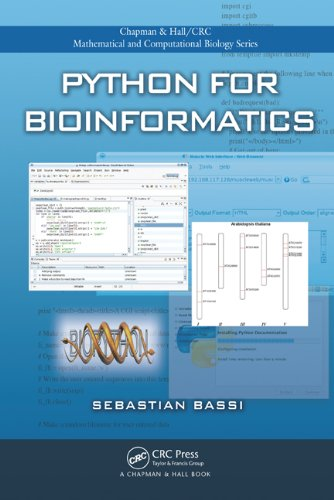
\includegraphics[width=.18\textwidth]{images/bassi_book}
	
\includegraphics[width=.2\textwidth]{images/korf_book}
	
\includegraphics[width=.2\textwidth]{images/model_book}
   \end{frame}

 %%%
 % SECTION: Recording your work
   \section{Recording Your Work}
   
   % SUBSECTION: justification
   \subsection{Why and How?}
   \begin{frame}
     \frametitle{Why Do It?}
     \begin{itemize}
	   \item Doing bioinformatics is doing science: keep a lab book!
	   \item You \emph{will not} remember multiple files, analysis details, etc. in a week/month/six months/a year/three years
	   \begin{itemize}
	     \item Noble (2009) \url{http://dx.doi.org/10.1371/journal.pcbi.1000424}
	     \item Baggerly \& Coombes (2009) \url{http://arxiv.org/pdf/1010.1092.pdf}
	   \end{itemize}
	\end{itemize}
	
\includegraphics[width=.6\textwidth]{images/noble_2009_head}
   \end{frame}
   
   \begin{frame}
     \frametitle{How To Do It? I}
     \begin{itemize}
	   \item There is no one correct way, but$\ldots$
	   \item Think about data/docs/project structure \textit{before} you start
	\end{itemize}
    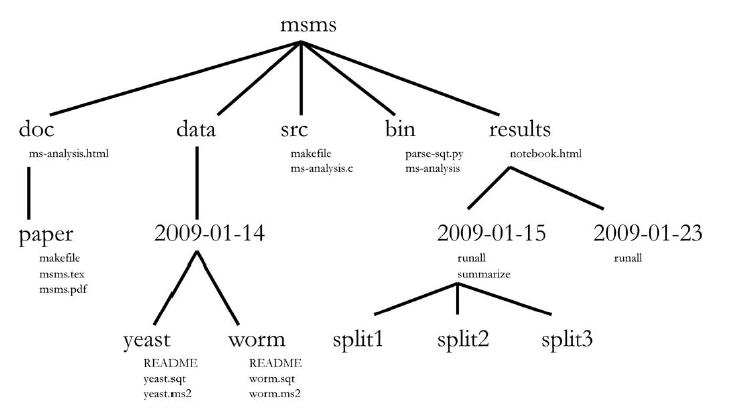
\includegraphics[width=.5\textwidth]{images/project_structure}
    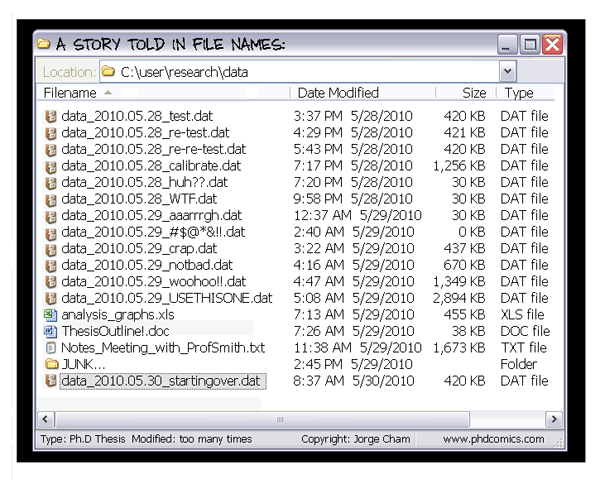
\includegraphics[width=.5\textwidth]{images/phd052810s}
   \end{frame}

   \begin{frame}
     \frametitle{How To Do It? II}
     \begin{itemize}
	   \item Use plain text where possible
	   \item Use version control
	   \item Keep backups
	   \item Different tools suit different purposes: code \textit{vs.} data \textit{vs.} analysis \textit{vs.} $\ldots$
	   \item Find a way that works \emph{for you}.
	\end{itemize}
   \end{frame}

   \begin{frame}
     \frametitle{How To Do It? III}
     \begin{itemize}
	   \item Reproducibility is key!
	   \item Scripts and pipelines are better for this than notes of what you did
	   \begin{itemize}
	     \item Also better for version control, and reuse
	   \end{itemize}
	   \item Avoid unnecessary duplication
	   \begin{itemize}
	     \item Someone else may have solved your problem
	     \item One (backed up) read-only copy of raw data, keep analyses separate
	   \end{itemize}
	\end{itemize}
   \end{frame}
   
   
   % SUBSECTION: useful tools
   \subsection{Useful Tools for Recording Your Work}
   \begin{frame}
     \frametitle{Plain Text Files}
     \begin{itemize}
       \item \texttt{README.txt}/\texttt{README.md} in each directory/folder
       \item Plain text is always human-readable
       \begin{itemize}
         \item Markdown (\url{https://daringfireball.net/projects/markdown/basics})
         \item RST (\url{http://docutils.sourceforge.net/docs/ref/rst/restructuredtext.html})
       \end{itemize}
     \end{itemize}
    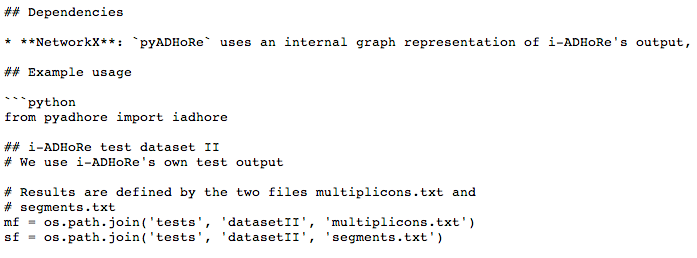
\includegraphics[width=.4\textwidth]{images/markdown_before}
	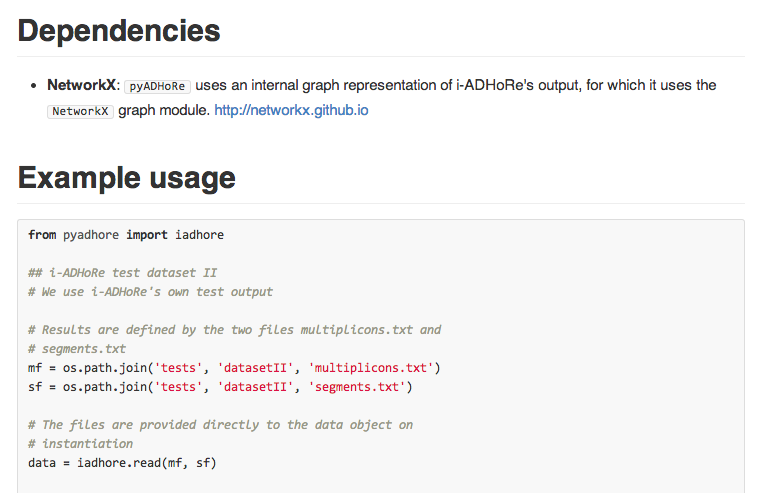
\includegraphics[width=.4\textwidth]{images/markdown_after}
   \end{frame}
   
   \begin{frame}
     \frametitle{Galaxy workflows}
     \begin{itemize}
       \item Use through browser, graphical interface
       \item Reproducible, shareable, documented, reusable analyses
       \item Wraps standard bioinformatics tools
       \item Local instance (\url{http://ppserver/galaxy}) uses JHI cluster       
     \end{itemize}
     \begin{center}
       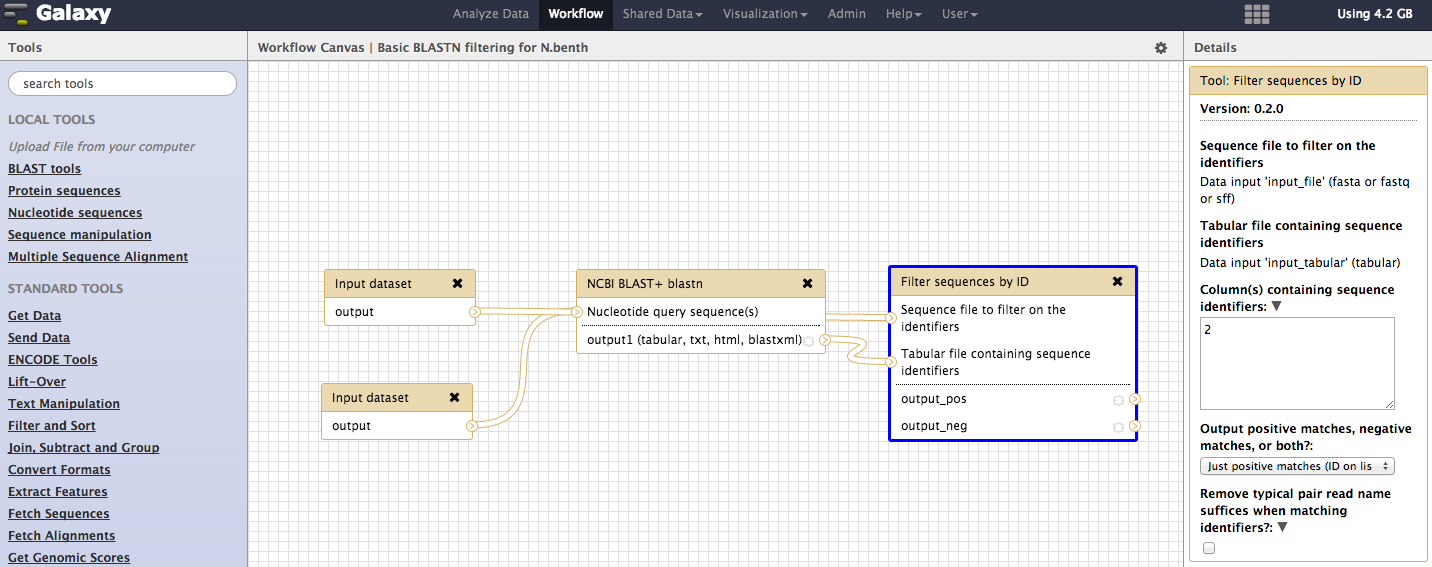
\includegraphics[width=.75\textwidth]{images/galaxy_screenshot}
     \end{center}
   \end{frame}      
   
   \begin{frame}
     \frametitle{\texttt{script}}
     \begin{itemize}
       \item Writes your terminal activity to a plain text file
       \item Saves effort copy/pasting and typing commands into a lab book, as you go
       \item Easy to use with other tools 
       \item use \texttt{man script} at your terminal to find out more
     \end{itemize}
   \end{frame}   
   
   \begin{frame}
     \frametitle{MediaWiki}
     \begin{itemize}
       \item Useful for shared projects/data
       \item Automatic version control and attribution
       \item Many local instances at JHI (ask around)
     \end{itemize}
    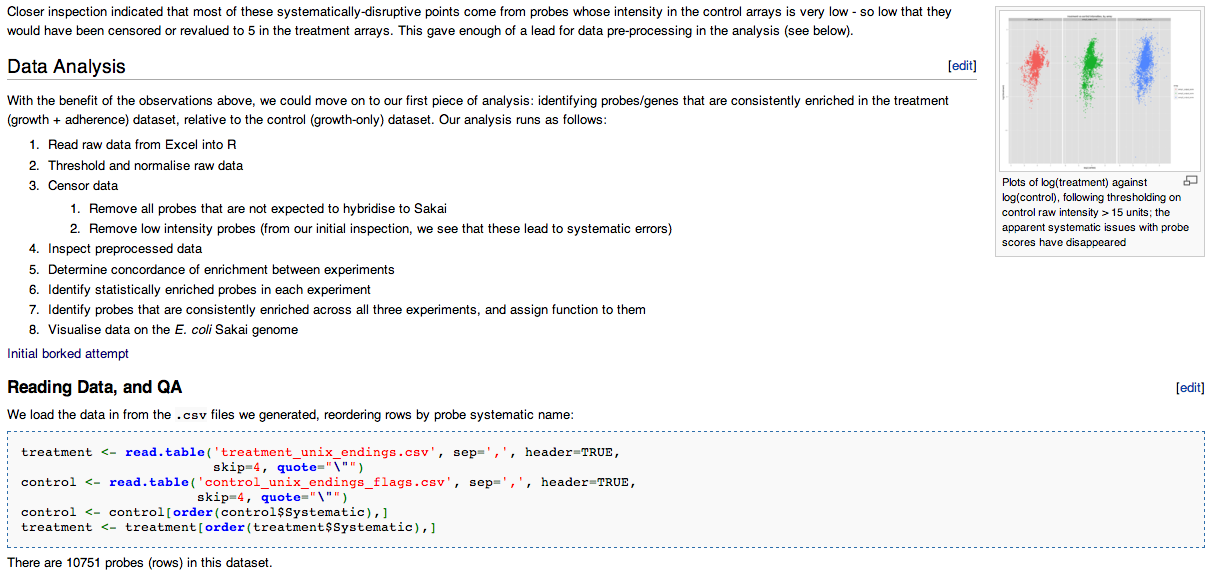
\includegraphics[width=.4\textwidth]{images/mediawiki_after}
	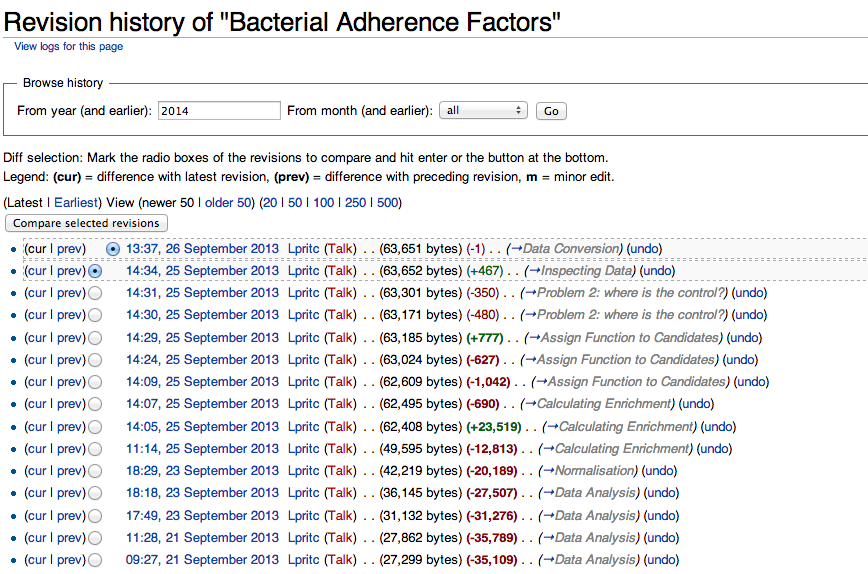
\includegraphics[width=.4\textwidth]{images/mediawiki_version_control}     
   \end{frame}
   
   \begin{frame}
     \frametitle{A language notebook}
     \begin{itemize}
       \item e.g. \texttt{iPython Notebook}, \texttt{Mathematica}, \texttt{MatLab} cells
       \item Integrates live code and analysis with lab-book
     \end{itemize}
    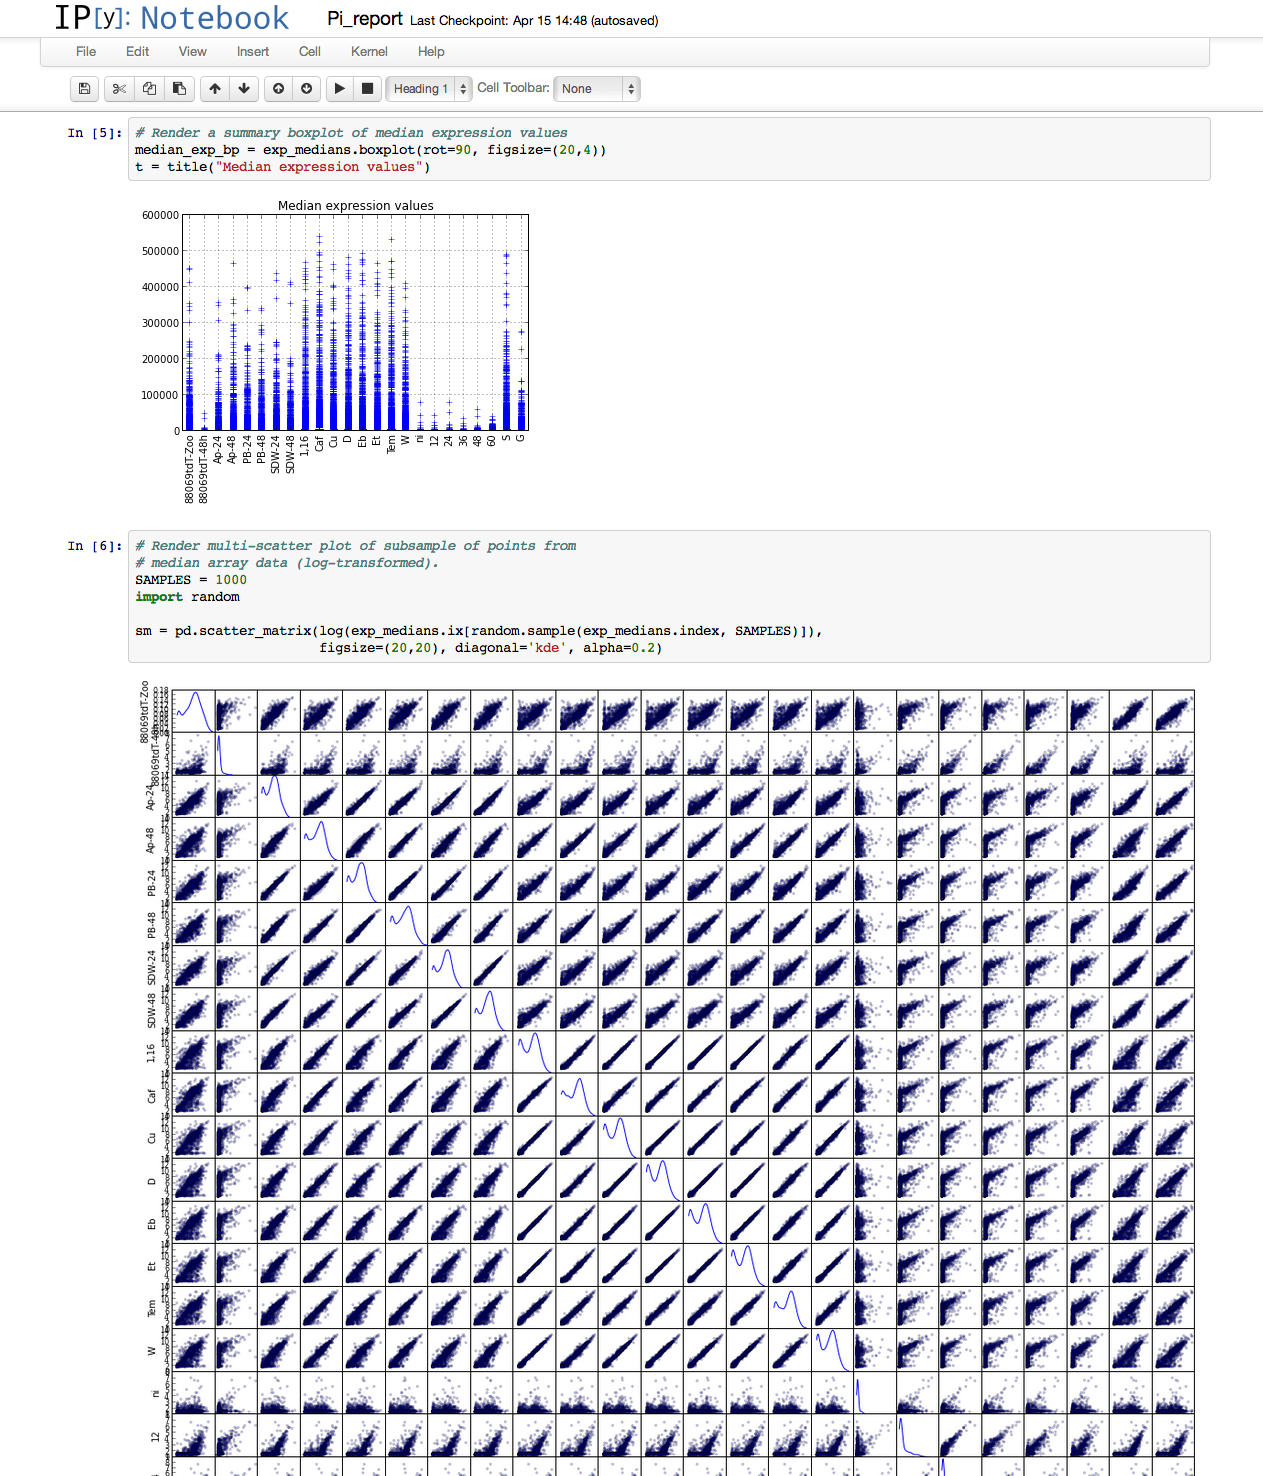
\includegraphics[width=.5\textwidth]{images/ipython_notebook}     
   \end{frame}

   \begin{frame}
     \frametitle{\LaTeX}
     \begin{itemize}
       \item Powerful, versatile typesetting system
       \item Similar to markup/markdown
       \item Pros: great for mathematical/computing work
       \item Cons: not user-friendly
     \end{itemize}
    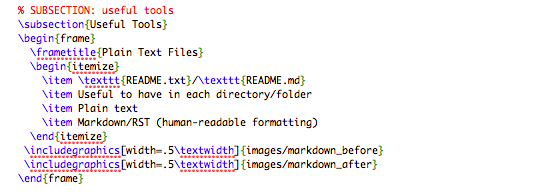
\includegraphics[width=.35\textwidth]{images/latex_before}
    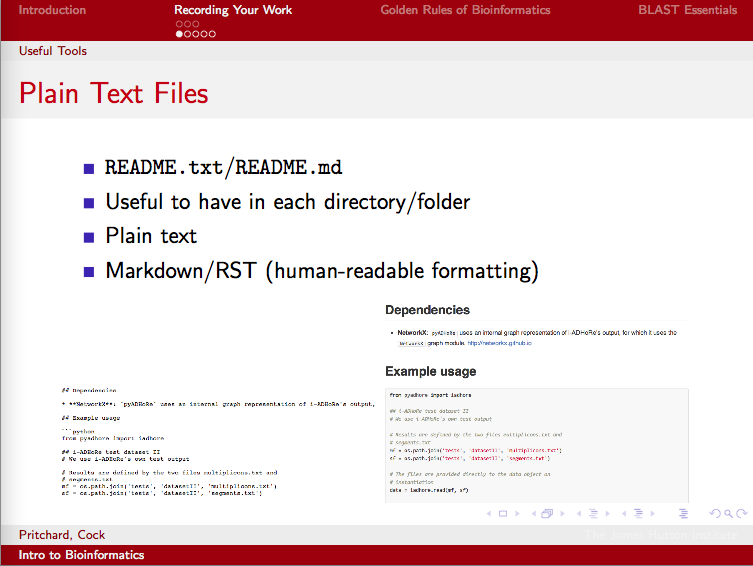
\includegraphics[width=.35\textwidth]{images/latex_after}     
   \end{frame}

 %%%
 % SECTION: The Golden Rules of Bioinformatics
  \section{Golden Rules of Bioinformatics}
  
  \subsection{Rule 1}
  \begin{frame}
    \frametitle{Exercise 1}
    \framesubtitle{Subgroups}
    \begin{itemize}
      \item You are in group A, B, C or D - this decides your dataset: \\
      \texttt{expnA.tab}, \texttt{expnB.tab}, \texttt{expnC.tab}, \texttt{expnD.tab}
      \item You will use \texttt{R} at the command-line to analyse your data
    \end{itemize}
  \end{frame}
  
  \begin{frame}
    \frametitle{Exercise 1}
    \framesubtitle{The biological question}
    \begin{itemize}
      \item Your dataset \texttt{expn?.tab} describes (log) expression data for two genes: \texttt{gene1} and \texttt{gene2}
      \item Expression measured at eleven time points (including control)
      \item Q: Are \texttt{gene1} and \texttt{gene2} genes coregulated?
      \item How do we answer this question?
    \end{itemize}
  \end{frame}  

  \begin{frame}
    \frametitle{Exercise 1}
    \framesubtitle{Reformulating the question}
    \begin{itemize}
      \item<1-> Q: Are \texttt{gene1} and \texttt{gene2} genes coregulated?
      \item<1-> A: We cannot determine this from expression data alone
      \item<2-> Reformulate the question:
      \item<2-> NewQ: Is there evidence that \texttt{gene1} and \texttt{gene2} expression profiles are correlated? \\
            (is expression \texttt{gene1} $\propto$ \texttt{gene2})
      \item<2-> How do we answer this new question?
    \end{itemize}
  \end{frame}

% [fragile] frames must end with \end{frame} directly following a newline, or they break!
  \begin{frame}[fragile]
    \frametitle{Exercise 1}
    \framesubtitle{Starting the analysis}
    \begin{itemize}
      \item Change directory to where Exercise 1 data is located, and start R.
    \end{itemize}
    \begin{lstlisting}[language=bash]
$ cd ../../data/ex1_expression/
$ R
    \end{lstlisting}
\end{frame}

% [fragile] frames must end with \end{frame} directly following a newline, or they break!
  \begin{frame}[fragile]
    \frametitle{Exercise 1}
    \framesubtitle{Load and inspect data in R}
    \begin{lstlisting}[language=R]
> data = read.table("expnA.tab", sep="\t", 
                    header=TRUE)
> head(data)
  gene1 gene2
1    10  8.04
2     8  6.95
3    13  7.58
4     9  8.81
5    11  8.33
6    14  9.96
    \end{lstlisting}
    %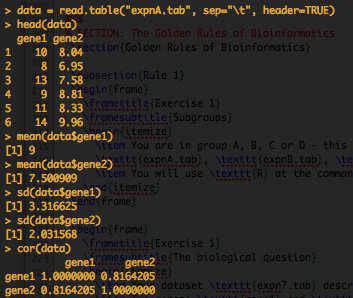
\includegraphics[width=.5\textwidth]{images/ex1_screenshot_b}
\end{frame}

% [fragile] frames must end with \end{frame} directly following a newline, or they break!
  \begin{frame}[fragile]
    \frametitle{Exercise 1}
    \framesubtitle{Load and inspect data in R}
    \begin{lstlisting}[language=R]
> mean(data$gene1)
[1] 9
> mean(data$gene2)
[1] 7.500909
> sd(data$gene1)
[1] 3.316625
> sd(data$gene2)
[1] 2.031568
> cor(data)
          gene1     gene2
gene1 1.0000000 0.8164205
gene2 0.8164205 1.0000000
    \end{lstlisting}
    %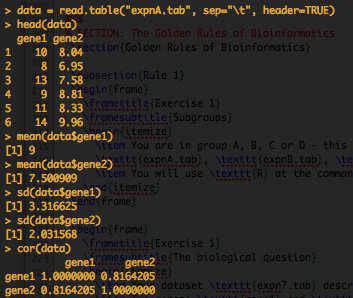
\includegraphics[width=.5\textwidth]{images/ex1_screenshot_b}
\end{frame}

  \begin{frame}
    \frametitle{Exercise 1}
    \framesubtitle{Results}
    \begin{center}
	\begin{tabular}{r|l|l|l|l}
	  measure & expnA & expnB & expnC & expnD \\
	  \hline
	  mean(gene1) & 9     &  &  & \\
	  mean(gene2) & 7.5   &  &  & \\
  	  sd(gene1)   & 3.3   &  &  & \\
  	  sd(gene1)   & 2.0   &  &  & \\  
	  cor(data)   & 0.816 &  &  & \\  
	\end{tabular}
    \end{center}
  \end{frame}

  \begin{frame}
    \frametitle{Exercise 1}
    \framesubtitle{Results}
    \begin{center}
	\begin{tabular}{r|l|l|l|l}
	  measure & expnA & expnB & expnC & expnD \\
	  \hline
	  mean(gene1) & 9     & 9     & 9     & 9 \\
	  mean(gene2) & 7.5   & 7.5   & 7.5   & 7.5 \\
  	  sd(gene1)   & 3.3   & 3.3   & 3.3   & 3.3 \\
  	  sd(gene1)   & 2.0   & 2.0   & 2.0   & 2.0 \\  
	  cor(data)   & 0.816 & 0.816 & 0.816 & 0.816 \\  
	\end{tabular}
	\end{center}
	\begin{itemize}
      \item<2-> $r=0.816 (P<0.005)$ in every experiment
      \item<2-> Can we conclude that \texttt{gene1} and \texttt{gene2} are coexpressed in each experiment?
    \end{itemize}
  \end{frame}

% [fragile] frames must end with \end{frame} directly following a newline, or they break!
  \begin{frame}[fragile]
    \frametitle{Exercise 1}
    \framesubtitle{Plot the data in R}
    Should have done this, first! \\
    \begin{lstlisting}[language=R]
> plot(data)
    \end{lstlisting}
    \begin{center}
      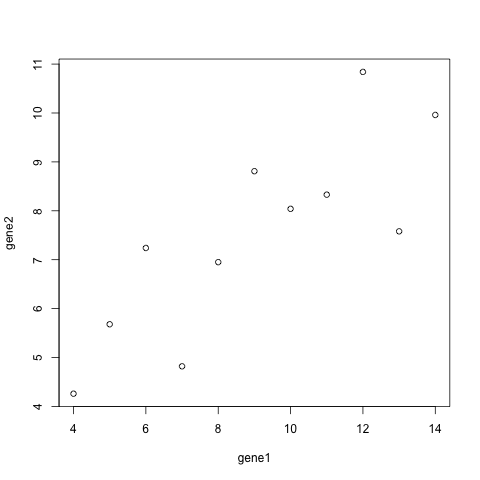
\includegraphics[width=0.4\textwidth]{images/ex1_screenshot_d}        
    \end{center}
\end{frame}

  \begin{frame}
    \frametitle{Exercise 1}
    \framesubtitle{Always plot the data}
    Which gene pairs are coexpressed?
    \begin{center}
      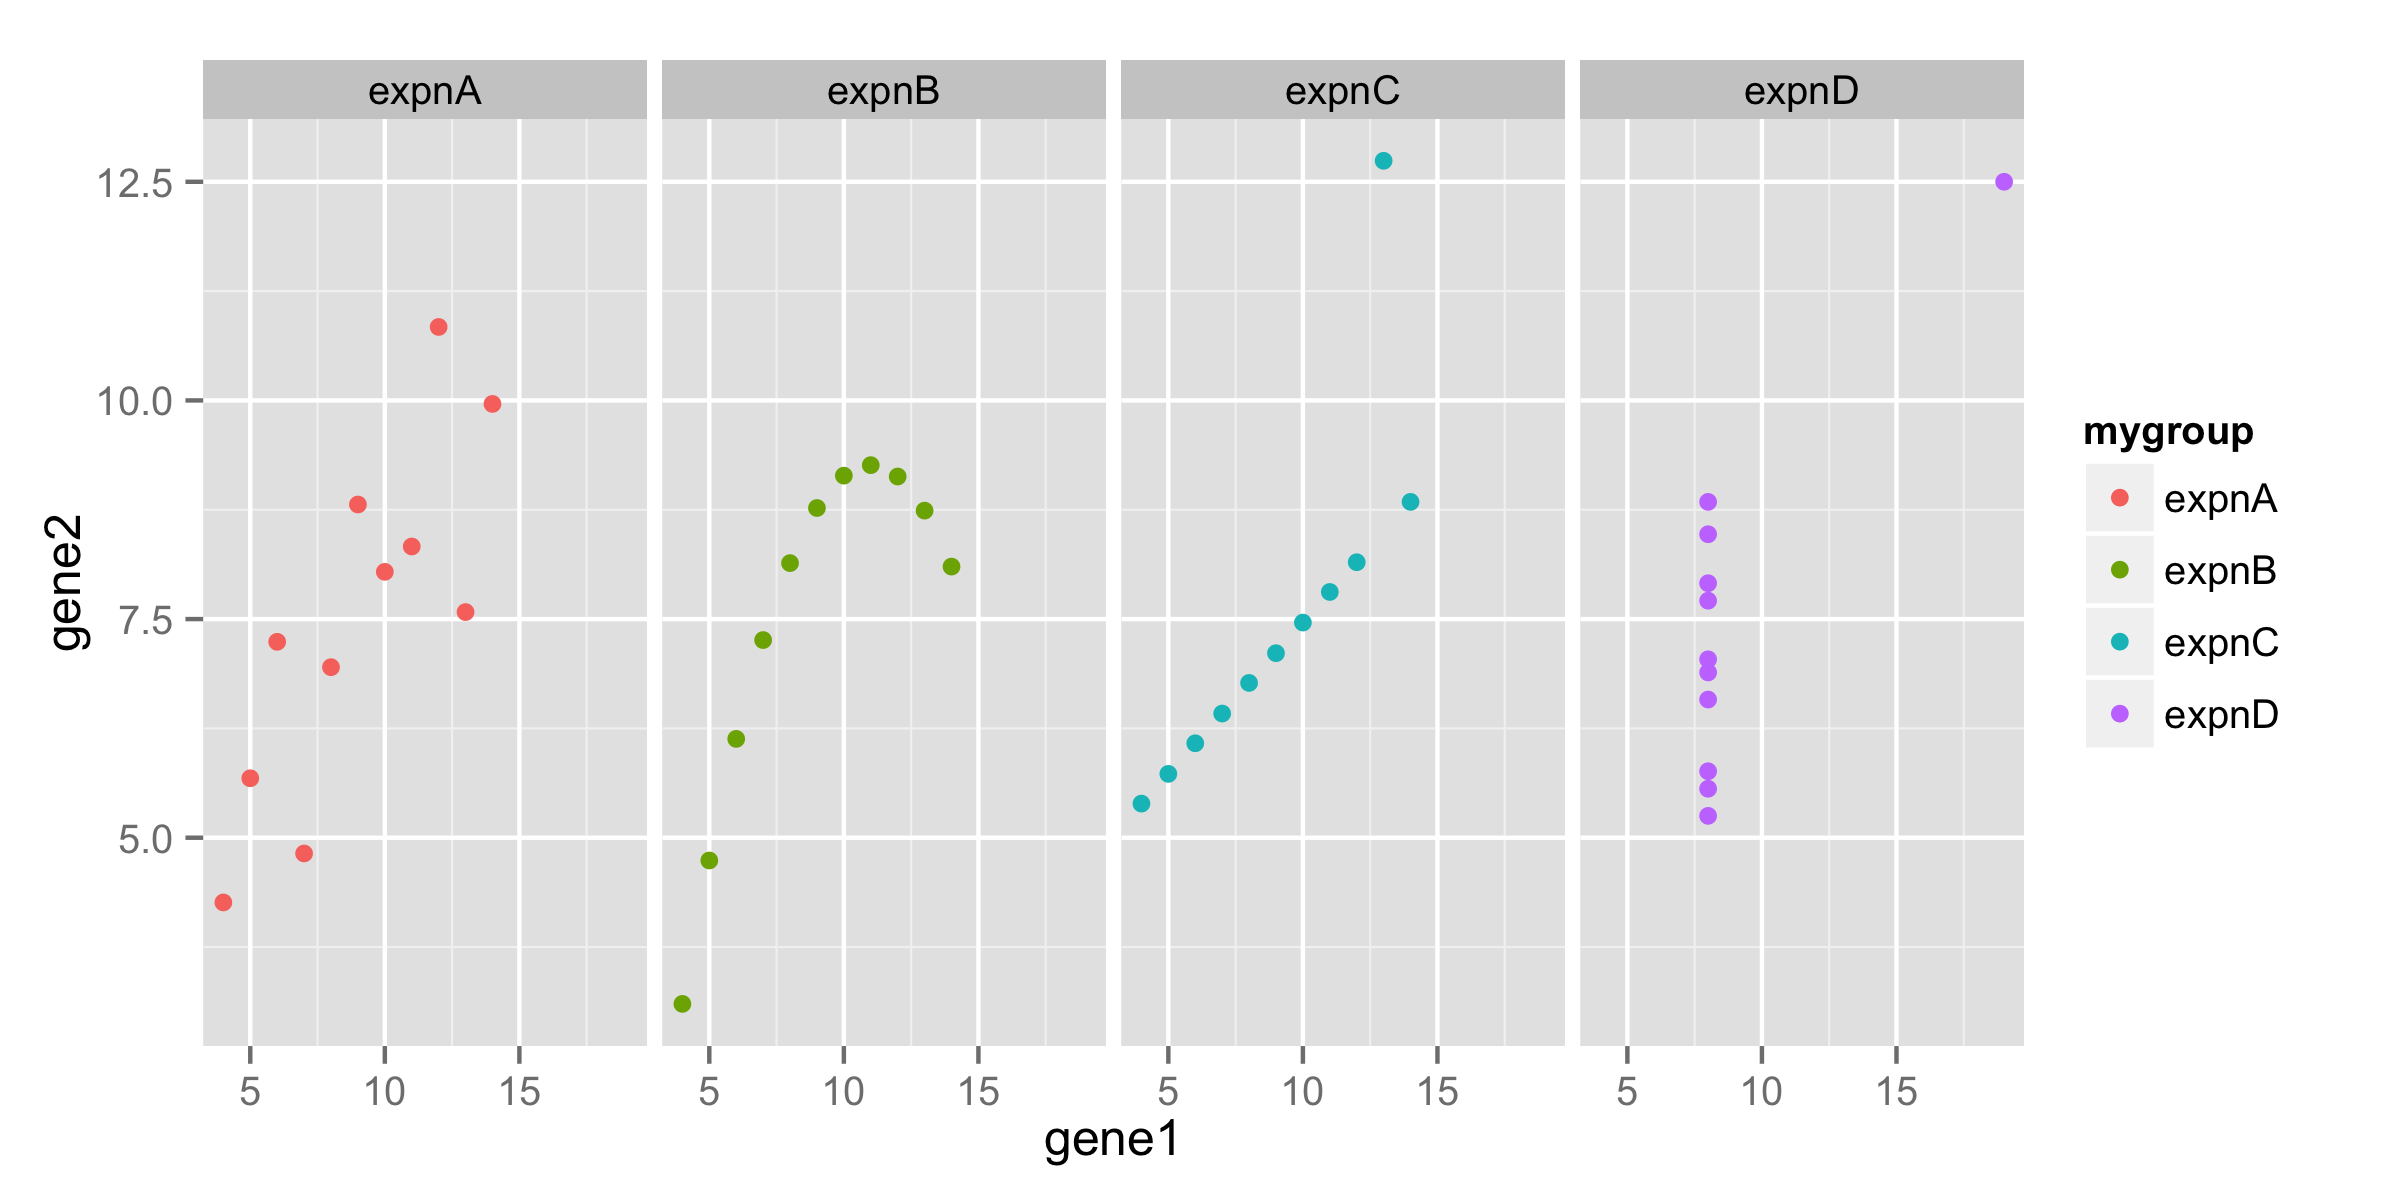
\includegraphics[width=0.9\textwidth]{images/ex1_rplot} \\
    \end{center}
  \end{frame}

  \begin{frame}
    \frametitle{First Golden Rule of Bioinformatics}
    \framesubtitle{Do not trust the data}
	\begin{itemize}
	  \item Always inspect the raw data (trends, outliers, clustering)
	  \item What is the question? Can the data answer it?
	  \item Communicate with data collectors! (don't be afraid of pedantry)
	  \begin{itemize}
	    \item Who? When? How?
	    \item You need to understand the experiment to analyse it (easier if you helped design it).
	    \item Be wary of block effects (experimenter, time, batch, etc.)
	  \end{itemize}
	\end{itemize}
  \end{frame}

  \subsection{Rule 2}
  \begin{frame}
    \frametitle{Exercise 2}
    \framesubtitle{Instructions}    
    \begin{itemize}
      \item You are in group A, B, C or D - this decides your database\\
      \texttt{dbA}, \texttt{dbB}, \texttt{dbC}, \texttt{dbD}
      \item You will use \texttt{BLAST} at the command-line to analyse your data
      \item You will use \texttt{script} at the command-line to record your work
    \end{itemize}
  \end{frame}

% [fragile] frames must end with \end{frame} directly following a newline, or they break!
  \begin{frame}[fragile]
    \frametitle{Exercise 2}
    \framesubtitle{Starting \texttt{script}}    
    \begin{itemize}
      \item Start recording your actions by entering \texttt{script} at the command line      
    \end{itemize}
    \begin{lstlisting}[language=bash]
$ script
Script started, output file is typescript
    \end{lstlisting}    
\end{frame}

% [fragile] frames must end with \end{frame} directly following a newline, or they break!
  \begin{frame}[fragile]
    \frametitle{Exercise 2}
    \framesubtitle{Running \texttt{BLAST}}
    \begin{itemize}
      \item Change directory to the \texttt{ex2\_blast} directory
      \item Run \texttt{BLAST} with the appropriate database
      \item Exit \texttt{script}
    \end{itemize}
    \begin{lstlisting}[language=bash]
$ cd ../ex2_blast
$ blastp -num_alignments 1 -num_descriptions 1 \
    -query query.fasta -db dbA
$ exit
exit
Script done, output file is typescript
    \end{lstlisting}    
\end{frame}

% [fragile] frames must end with \end{frame} directly following a newline, or they break!
  \begin{frame}[fragile]
    \frametitle{Exercise 2}
    \framesubtitle{Viewing \texttt{script} output}
    \begin{itemize}
      \item You can view the \texttt{typescript} file with \texttt{cat}
    \end{itemize}
    \begin{lstlisting}[language=bash]
$ cat typescript
Script started on Fri May  9 10:45:12 2014
lpritc@lpmacpro:$ cd ../ex2_blast
[...]
    \end{lstlisting}    
\end{frame}

% [fragile] frames must end with \end{frame} directly following a newline, or they break!
  \begin{frame}[fragile]
    \frametitle{Exercise 2}
    \framesubtitle{\texttt{BLAST} output}
    \begin{tiny}
    \begin{verbatim}
Query= query protein sequence

Length=400
                                                                      Score
Sequences producing significant alignments:                          (Bits)

  PITG_08491T0 Phytophthora infestans T30-4 choline transporter-l...  34.3


> PITG_08491T0 Phytophthora infestans T30-4 choline transporter-like 
protein (441 aa)
Length=486

 Score = 34.3 bits (77), Method: Compositional matrix adjust.
 Identities = 22/69 (32%), Positives = 38/69 (55%), Gaps = 4/69 (6%)

Query  106  EVILPMMYQFALKPSFADVINDYKPYSKHTAGVSDQELKGEATTWMLADKNSRMKAFLSQ  165
            E+++PM+Y   L   F   ++ Y P   HTA ++  EL+G   T ++A+  S +  F ++
Sbjct  40   ELMVPMLYSLYLVVLFHLPVSAYYP---HTASMTAHELQGAVITILVAETPSIIIQF-AK  95

Query  166  IKTKSNSSE  174
              T SN S+
Sbjct  96   CHTSSNISQ  104
    \end{verbatim}   
    \end{tiny} 
\end{frame}

  \begin{frame}
    \frametitle{Exercise 2}
    \framesubtitle{Results}
    \begin{itemize}
      \item What is a reasonable E-value threshold to call a 'match'?
      \begin{itemize}
        \item 1e-05, 0.001, 0.1, 10?
      \end{itemize}
    \end{itemize}
    \begin{center}
	\begin{tabular}{r|l|l|l|l}
	   & dbA & dbB & dbC & dbD \\
	  \hline
	  \hline
	  E-value &      &  &  & \\
	\end{tabular}
    \end{center}
  \end{frame}

  \begin{frame}
    \frametitle{Exercise 2}
    \framesubtitle{Results}
    \begin{itemize}
      \item What is a reasonable E-value threshold to call a 'match'?
      \begin{itemize}
        \item 1e-05, 0.001, 0.1, 10?
      \end{itemize}
    \end{itemize}
    \begin{center}
	\begin{tabular}{r|l|l|l|l}
	   & dbA & dbB & dbC & dbD \\
	  \hline
	  \hline
	  E-value & 0.45 & 0.002 & 4e-06 & 0.019 \\
	\end{tabular}
    \end{center}
    \begin{itemize}
      \item Five orders of magnitude difference in E-value, depending on database choice - Why?
    \end{itemize}    
  \end{frame}

  \begin{frame}
    \frametitle{Exercise 2}
    \framesubtitle{Results}
    \begin{itemize}
      \item E-values depend on database size
      \item Bit score and alignment do not depend on database size
    \end{itemize}
    \begin{center}
	\begin{tabular}{r|l|l|l|l}
	   & dbA & dbB & dbC & dbD \\
	  \hline
	  \hline
	  E-value & 0.45 & 0.002 & 4e-06 & 0.019 \\
	  Bit score & 34.3 & 34.3 & 34.3 & 34.3 \\
	  \hline
	  Sequences & 100,001 & 501 & 1 & 5,001 \\
	  Letters & 48,650,486 & 210,866 & 486 & 2,066,510 	  
	\end{tabular}
    \end{center}
  \end{frame}

  \begin{frame}
    \frametitle{Exercise 2}
    \framesubtitle{Results}    
    \begin{itemize}
      \item<1-> E-values differ, but the query matches a choline transporter-like 
protein quite well
      \item<2-> Doesn't it?
    \end{itemize}
  \end{frame}

% [fragile] frames must end with \end{frame} directly following a newline, or they break!
  \begin{frame}[fragile]
    \frametitle{Exercise 2}
    \framesubtitle{\texttt{BLAST} output}
    \begin{tiny}
    \begin{verbatim}
Query= query protein sequence

Length=400
                                                                      Score     E
Sequences producing significant alignments:                          (Bits)  Value

  PITG_08491T0 Phytophthora infestans T30-4 choline transporter-l...  34.3    4e-06


> PITG_08491T0 Phytophthora infestans T30-4 choline transporter-like 
protein (441 aa)
Length=486

 Score = 34.3 bits (77),  Expect = 4e-06, Method: Compositional matrix adjust.
 Identities = 22/69 (32%), Positives = 38/69 (55%), Gaps = 4/69 (6%)

Query  106  EVILPMMYQFALKPSFADVINDYKPYSKHTAGVSDQELKGEATTWMLADKNSRMKAFLSQ  165
            E+++PM+Y   L   F   ++ Y P   HTA ++  EL+G   T ++A+  S +  F ++
Sbjct  40   ELMVPMLYSLYLVVLFHLPVSAYYP---HTASMTAHELQGAVITILVAETPSIIIQF-AK  95

Query  166  IKTKSNSSE  174
              T SN S+
Sbjct  96   CHTSSNISQ  104
    \end{verbatim}   
    \end{tiny} 
\end{frame}

  \begin{frame}
    \frametitle{Exercise 2}
    \framesubtitle{Remember Golden Rule 1?}    
    \begin{itemize}
      \item<1-> Sequence accessions (\texttt{PITG\_?????T0}) \emph{are} correct in the databases
      \item<2-> Sequence functional descriptions are randomly shuffled: lengths do not match in \texttt{BLAST} output
      \item<3-> \texttt{dbA} contains only three different sequences: two are repeated 50,000 times
      \item<4-> \texttt{query.fasta} is random sequence, not a real protein
      \begin{itemize}
        \item<4-> Shuffled from all \textit{P. infestans} proteins
        \item<4-> No \texttt{nr} or \texttt{PFam} matches        
      \end{itemize}
    \end{itemize}
  \end{frame}

  \begin{frame}
    \frametitle{Second Golden Rule of Bioinformatics}
    \framesubtitle{Do not trust the software}
	\begin{itemize}
	  \item Do not trust the software
	  \item You must understand the analysis/algorithm
	  \item Always sanity test
	  \item Test output for robustness to parameter choice
	  \item Remember:
	  \begin{itemize}
	    \item Software has bugs
	    \item Algorithms have assumptions, conditions, and applicable domains
	    \item Some problems are inherently hard, or even insoluble
	  \end{itemize}
	\end{itemize}
  \end{frame}

  \subsection{Rule 3}  
  \begin{frame}
    \frametitle{Exercise 3}
    \framesubtitle{Classification}
    \begin{itemize}
      \item Rule: If there is a vowel on one side of the card, there \textit{must} be an even number on the other side.
      \item Which cards \textit{must} be turned over to determine if the rule holds true? (How many, and which ones)
    \end{itemize}
    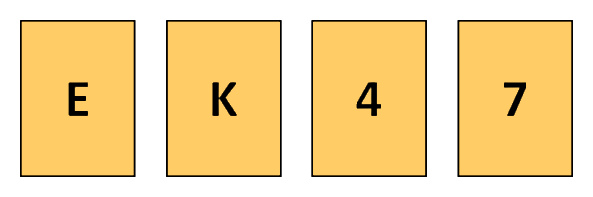
\includegraphics[width=0.8\textwidth]{images/wason}
  \end{frame}

  \begin{frame}
    \frametitle{Exercise 3}
    \framesubtitle{Classification}
    \begin{itemize}
      \item This is equivalent to protein functional classification
      \item Rule: If there is a CRN/RxLR/T3SS domain, the protein \textit{must} be an effector.
    \end{itemize}
    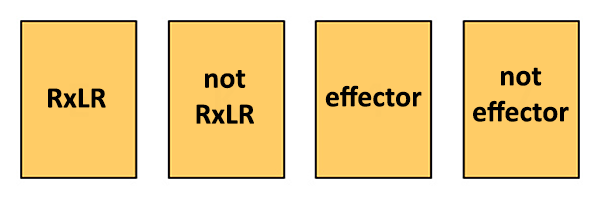
\includegraphics[width=\textwidth]{images/wason_rxlr}
  \end{frame}

  \begin{frame}
    \frametitle{Exercise 3}
    \framesubtitle{Classification}
    \begin{itemize}
      \item<1-> If you chose \emph{E} and \emph{4}
      \begin{itemize}
        \item<2-> You are in the typical majority group
        \item<3-> You are not correct
        \item<4-> You have been a victim of confirmation bias (System 1 thinking)
      \end{itemize}
      \item<5-> If you chose \emph{E} and \emph{7}
      \begin{itemize}
        \item<6-> Congratulations!
        \item<6-> Your choice was capable of \textit{falsifying} the rule.
      \end{itemize}
    \end{itemize}
  \end{frame}

  \begin{frame}
    \frametitle{Exercise 3}
    \framesubtitle{Classification}
    \begin{center}
	\begin{tabular}{c|c|c}
	  Card & Outcome & Rule \\
	  \hline
	  \hline
	    \multirow{2}{*}{E} & Even & True \emph{for this card} \\
	                                & Odd & \emph{violated} \\
	  \hline
	    \multirow{2}{*}{K} & Even & na \\
	                                & Odd & na \\	    
	  \hline
	    \multirow{2}{*}{4} & Vowel & True \emph{for this card} \\
	                                & Consonant & na \\
	  \hline
	    \multirow{2}{*}{7} & Vowel & \emph{violated} \\
	                                & Consonant & na \\	    
	\end{tabular}
    \end{center}
  \end{frame}

  \begin{frame}
    \frametitle{Third Golden Rule of Bioinformatics}
    \framesubtitle{Don't trust yourself}
	\begin{itemize}
	  \item Everyone has expectations of their data/experiment
	    \begin{itemize}
	      \item Beware cognitive errors, such as confirmation bias!
	      \item System 1 vs. System 2 $\approx$ reason vs. intuition
	    \end{itemize}
	  \item Think statistically! 
	    \begin{itemize}
	      \item Large datasets can be counterintuitive.
	      \item Always account for multiple tests.
	    \end{itemize}
	  \item Use test-driven development of analyses and code
	    \begin{itemize}
	      \item Use examples that pass \textit{and} fail
	    \end{itemize}	  
	\end{itemize}
  \end{frame}


%%%
% SECTION: 
  \section{}

  \begin{frame}
    \frametitle{Third Golden Rule of Bioinformatics}
    \framesubtitle{Keep raw data and analysis separate}
	\begin{itemize}
	  \item Keep raw data and analysis separate
	  \item Avoid Excel! (off-by-one/copy errors/risk of changing data)
	  \item Make raw data read-only, and back it up immediately
	\end{itemize}
  \end{frame}


  \begin{frame}
    \frametitle{Programming}
   % \framesubtitle{Keep raw data and analysis separate}
	\begin{itemize}
	  \item Programming is like writing a book$\ldots$
	  \item $\ldots$except that if you miss out a comma on p.126, the whole thing makes no damned sense!
	\end{itemize}
  \end{frame}

  \begin{frame}
    \frametitle{Assessing Performance}
    \framesubtitle{Contingency Tables}
    \begin{center}
	\begin{tabular}{cc|c|c|}
	  \cline{3-4}
		& & \multicolumn{2}{|c|}{Condition (Gold standard)}\\
	  \cline{3-4}
		& & True & False \\
	  \hline
	  \multicolumn{1}{ |c| }{\multirow{2}{*}{Test outcome}}& 
	  \multicolumn{1}{ |c| }{Positive} & True Positive \cellcolor{green} & 
	    False Positive\cellcolor{red}\\
	  \cline{2-4}
	  \multicolumn{1}{ |c| }{} & \multicolumn{1}{ |c| }{Negative} & 
	    False Negative\cellcolor{red} & True Negative \cellcolor{green}\\
	  \hline
	\end{tabular}
	\end{center}
  \end{frame}

  \begin{frame}
  \end{frame}

% etc
\end{document}